The structural integrity of fuel and cladding materials under irradiation, thermal cycling, and corrosion is a critical constraint in reactor design. Neutronics performance controls reactivity and the effective use of fuel; however, material damage affects safety margins and operational lifetime. This section of the report presents the use of a multiphysics modeling framework to simulate fuel-cladding performance in the Last Breath Reactor (LBR) with the primary focus being on thermal gradients, stress evolution and damage mechanisms.

\subsection{Modeling Framework: Use of MOOSE}
The Multiphysics Object-Oriented Simulation Environment (MOOSE), developed by Idaho National Laboratory, was used to model the coupled thermomechanical and fracture behavior of the fuel–cladding system. MOOSE enables the solution of strongly coupled nonlinear partial differential equations using the finite element method within a modular, extensible framework.

MOOSE was chosen primarily for its ability to simulate coupled heat conduction and solid mechanics within a single simulation environment. Moreover, MOOSE supports custom material models, including corrosion-induced property degradation and eigenstrain contributions. This was essential, as it enabled the simulation of accurate estimates of material property degradation caused by the extreme thermo-mechanical stresses that PWR fuel generally experiences during heating and cooling. Afterward, a realistic variant of a damaged spent fuel pin was simulated through a reheating cycle in the Last Breath Reactor to test its survivability and failure limits.


\subsection{Governing Physics and Equations}
Using the Multiphysics framework of MOOSE the thermo-mechanical behavior of the fuel cladding system was modeled. The coupled framework integrated heat conduction, solid mechanics, creep deformation, corrosion and fracture. Below are the governing equations and corresponding assumptions that modeled this simulation

\paragraph{Heat Conduction}
The temperature distribution within the fuel pellet is governed by the heat conduction equation:
\begin{equation}
    \rho c_p\frac{\partial T}{\partial t}=\nabla\cdot\left(k_{\mathrm{eff}}\nabla T\right)+Q
\end{equation}
Due to volumetric heat generation from fission, strong radial temperature gradients develop, with peak temperatures occurring at the fuel centerline. Heat transfer occurs radially outwards towards the cladding where a convective heat flux boundary condition is established. As for the cooling phase, the heat generation term is reduced to zero.

\paragraph{Solid Mechanics}
Mechanical equilibrium is described by:
\begin{equation}
    \nabla\cdot \sigma + b =0
\end{equation}

where $\sigma$ is the Cauchy stress tensor (Pa), and $b$ represents body forces, which are assumed to be negligible in this study.

Since the scope of these simulations covers a 2D axisymmetric radial geometry, the stresses that make up the stress tensor are the radial and hoop stresses.

The hoop stress ($\sigma_\theta$) is described by:
\begin{equation}
    \sigma_\theta = \sigma_\theta(r)
\end{equation}

where:
\begin{itemize}
	\item $\sigma_\theta$ is the hoop (circumferential) stress (Pa),
	\item $r$ is the radial position (m).
\end{itemize}

The radial stress ($\sigma_r$) is described by:
\begin{equation}
    \sigma_r = \sigma_r(r)
\end{equation}

where:
\begin{itemize}
	\item $\sigma_r$ is the radial stress (Pa),
	\item $r$ is the radial position within the fuel--cladding system (m).
\end{itemize}

The total strain ($\varepsilon$) is decomposed as:
\begin{equation}
    \varepsilon = \varepsilon_e + \varepsilon_{th} + \varepsilon_{cr}\quad ,
\end{equation}
where $\varepsilon_e$ is the elastic strain, $\varepsilon_{th}$ is the thermal strain, and $\varepsilon_{cr}$ is the creep strain.

Here, the elastic response follows a linear isotropic Hooke's Law
\begin{equation}
    \varepsilon_r = \frac{1}{E} \left( \sigma_r - \nu \sigma_\theta \right)
\end{equation}

\begin{equation}
    \varepsilon_\theta = \frac{1}{E} \left( \sigma_\theta - \nu \sigma_r \right)
\end{equation}

where:
\begin{itemize}
	\item $\varepsilon_r$, $\varepsilon_\theta$ are the radial and hoop strains (-),
	\item $\sigma_r$, $\sigma_\theta$ are the radial and hoop stresses (Pa),
	\item $E$ is Young’s modulus (Pa),
	\item $\nu$ is Poisson’s ratio (-).
\end{itemize}

while thermal strain is computed by:
\begin{equation}
    \varepsilon_{th}=\alpha\left(T-T_\text{ref}\right)\mathbf{I}
\end{equation}

Where,  $\alpha$ is the coefficient of thermal expansion (1/K), $T_\text{ref}$ is the reference temperature, and $\mathbf{I}$ is the identity tensor. The mismatch in expansion rates between fuel and cladding induces stresses, leading to pellet-clad interaction (PCI).

Meanwhile, the creep strain is modeled by a Norton-type power law creep formulation with Arrhenius temperature dependence:

\begin{equation}
    \dot{\varepsilon}_{cr}=A\sigma_{\text{vm}}^{n}\exp{\left(-\frac{Q}{RT}\right)}
\end{equation}

where:
\begin{itemize}
	\item ${\dot{\varepsilon}}_{cr}$ is the creep strain rate (1/s),
	\item $A$ is a material constant,
	\item $\sigma_{vm}$ is the Von Mises equivalent stress (Pa),
	\item $n$ is the stress exponent,
	\item $Q$ is the activation energy (J/mol),
	\item $R$ is the universal gas constant (J/mol$\cdot$K),
	\item $T$ is temperature (K).
\end{itemize}

The Von Mises stress, $\sigma_{vm}$, is an equivalent stress derived from the distortion energy in a material. In this study, it is an overall stress state contributed by the hoop and radial stresses that drives the creep mechanism in the material.

\begin{equation}
    \sigma_{\text{vm}} = \sqrt{\sigma_r^2 - \sigma_r \sigma_\theta + \sigma_\theta^2}
\end{equation}

where:
\begin{itemize}
	\item $\sigma_{\text{vm}}$ is the Von Mises equivalent stress (Pa),
	\item $\sigma_r$ is the radial stress (Pa),
	\item $\sigma_\theta$ is the hoop (circumferential) stress (Pa).
\end{itemize}

This formulation captures the strong dependence of creep on both stress and temperature, making it particularly important under high-temperature conditions experienced in the Last Breath Reactor (LBR) cycle.

The overall thermal strain and stress drive the phase field to initiate crack propagation, which is modeled by Allen-Cahn:

\begin{equation}
    \frac{\partial\phi}{\partial t}=-L\frac{\delta F}{\delta\phi}\quad,
\end{equation}

where $\phi$ is the phase-field damage variable (0 = intact, 1 = fully fractured), $L$ is a mobility parameter, and $F$ is the total free energy functional.

Although this model was not used in the final Last Breath Reactor simulation, it was necessary to use it in the primary heating cycle to induce cracks in the fuel which would degrade the thermal conductivity. The model has also partially, i.e. at a small portion of the entire cycle timeline, been used in the LBR cycle to check for cladding rupture. The crack propagation is strongly coupled to thermal stress fields generated during reactor operation.

Meanwhile, for the cladding that is exposed to water for such a long time, a Arrhenius, temperature coupled corrosion model was applied

\begin{equation}
    x\left(t\right)=k_0\exp{\left(-\frac{Q}{RT}\right)}t^n
\end{equation}

where:
\begin{itemize}
	\item $x(t)$ is oxide thickness (m),
	\item $k_0$ is a rate constant,
	\item $Q$ is activation energy,
	\item $T$ is temperature,
	\item $n$ is a time exponent.
\end{itemize}

With a property degradation model of,
\begin{equation}
    D\left(T,t\right)=\operatorname{D}_0\exp{\left(-A\exp{\left(-\frac{\operatorname{Q}}{RT}\right)}t\right)}
\end{equation}

Where, D is a parameter such as conductivity, stiffness (Young’s modulus) etc. is degraded based on the corrosion.

\subsection{Modeling Assumptions}

To ensure computational tractability while capturing the dominant physical behavior, the following assumptions are made:
\begin{itemize}
    \item The problem is modeled in a 2D axisymmetric geometry, representing a radial cross-section of the fuel rod.
    \item Heat generation is applied only within the fuel region and is spatially uniform.
    \item Decay heat is neglected as it makes up about 7\% of the total reactor heat generation and decreases with time. 
    \item Mechanical behavior is quasi-static, with inertial effects neglected.
    \item Irradiation-induced swelling and fission gas release are neglected. However, for this model, these effects were ignored due to a relatively shorter operational cycle length for which the irradiation damage would be secondary to the thermo-mechanical damages \cite{Sweet2016BISONProperties}.%(Oak Ridge National Laboratory, Radiation Effects in Structural Materials, ORNL Report, 2017.: https://info.ornl.gov/sites/publications/files/Pub69721.pdf).
    \item Corrosion is temperature-driven and occurs only on exposed cladding surfaces.
    \item Material properties degrade as functions of temperature, stress, and damage but remain isotropic.
    \item The fuel gas gap was neglected in the simulations to ensure a tight configuration which occurs generally at the end of cycle for most PWR fuel \cite{Barrett2012AdvancedStudy}.%(U.S. Department of Energy, Advanced LWR Nuclear Fuel Cladding System Development Trade Study, 2012. [Online]. Available: https://www.energy.gov/ne/articles/advanced-lwr-nuclear-fuel-cladding-system-development-trade-study). 
\end{itemize}


These assumptions allow the model to focus on the dominant coupling between thermal gradients, stress evolution, creep deformation, corrosion, and fracture, which govern the structural integrity of the fuel–cladding system under LBR conditions.

\subsection{Primary heating cycle}
Simulations were modeled using the fuel material properties from Three Mile Island (TMI) Unit 1. The fuel was heated to a volumetric heat of 271 MW/m$^3$ under convective heat-flux boundary conditions.
Simulation results indicate the presence of strong radial temperature gradients within the fuel pellet, with centerline temperatures exceeding 1100 K and outer surface temperatures near 480 K. This is a characteristic behavior of UO$_2$ fuel due to the fuel having a relatively lower thermal conductivity than the cladding, which limits radial heat transport and this becomes the primary driver of stress development within the system.

\begin{figure}[H]
    \centering
    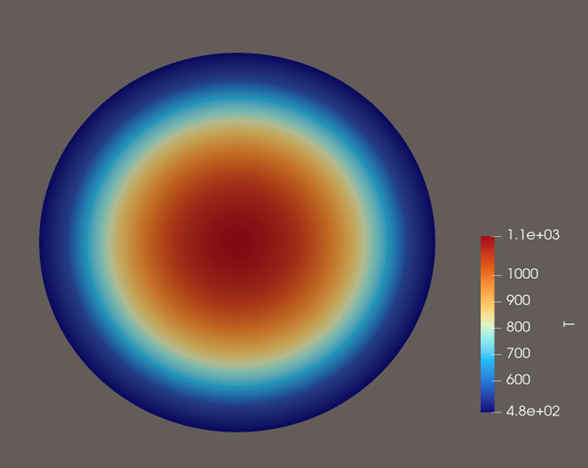
\includegraphics[width=0.5\linewidth]{figs/radial_heat_first_cycle.png}
    \caption{Radial Temperature profile in Kelvins for the first heating cycle at steady state.}
    \label{fig:placeholder}
\end{figure}

At the same time, the induced thermal expansion generates a significant mechanical stress due to the containment by the cladding. With the hoop stress profile it can be observed that there are compressive stresses in the fuel centerline and tensile stresses near the fuel-cladding interface. This is a direct consequence of the differential thermal expansion where the hot fuel expands relatively a lot more than the cooler cladding that leads to PCI.

\begin{figure}[H]
    \centering
    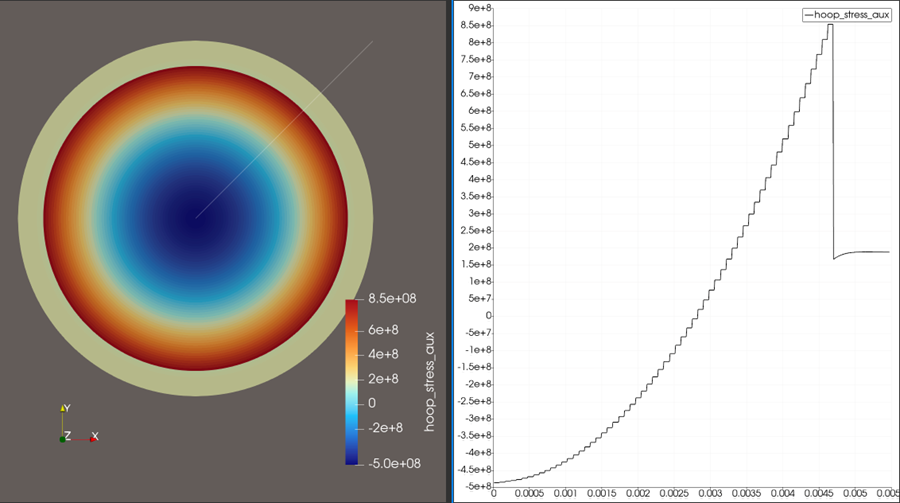
\includegraphics[width=0.6\linewidth]{hoopstress-ss.png}
    \caption{Hoop stress (Pa) at steady state }
    \label{fig:placeholder}
\end{figure}

The radial stress on the other hand helps monitor the compressive contact pressure between the cladding and the fuel. A high value at the fuel cladding interface during PCI indicates a high risk of plastic deformation and creep.

\begin{figure}[H]
    \centering
    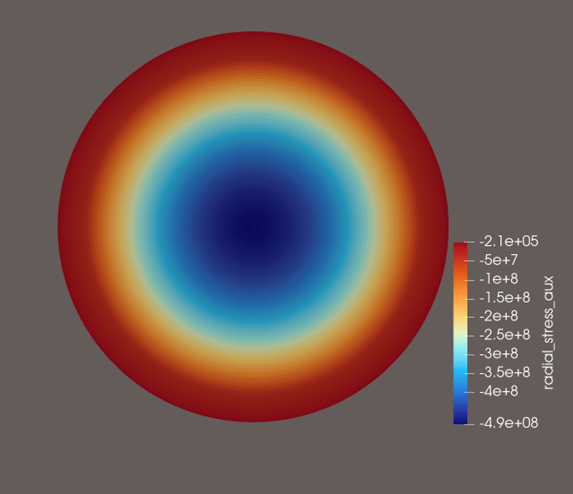
\includegraphics[width=0.5\linewidth]{figs/radial-stress-ss.png}
    \caption{The radial stress profile (Pa) at steady state.}
    \label{fig:placeholder}
\end{figure}
The hoop stresses and the radial stresses together contribute an overall stress state that yields the Von Mises stress, which mainly drives the creep mechanism that takes place during the cycle. This stress has a high value in the center of the fuel, which due to its ceramic properties undergoes constant deformation throughout the cycle. For the cladding on the other hand the stress is comparatively lower but still high enough to drive creep in the cladding region. As a result, the cladding is quite susceptible to failure by creep when it is eventually reheated in the LBR cycle.

\begin{figure}[H]
    \centering
    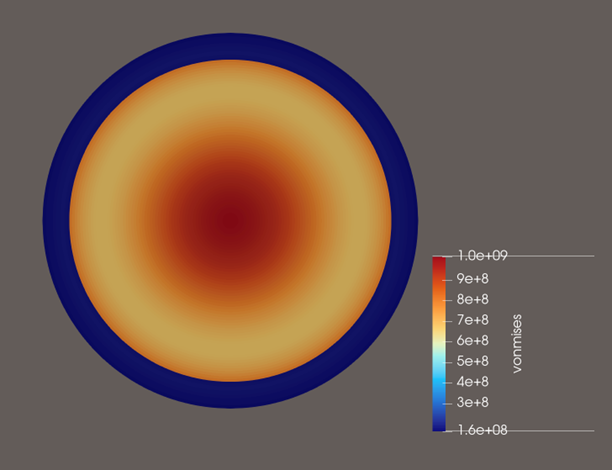
\includegraphics[width=0.5\linewidth]{figs/von-mises-ss-tmi1.png}
    \caption{Von Mises Stress profile at steady state during the operation of TMI-1.}
    \label{fig:placeholder}
\end{figure}

\begin{figure}[H]
    \centering
    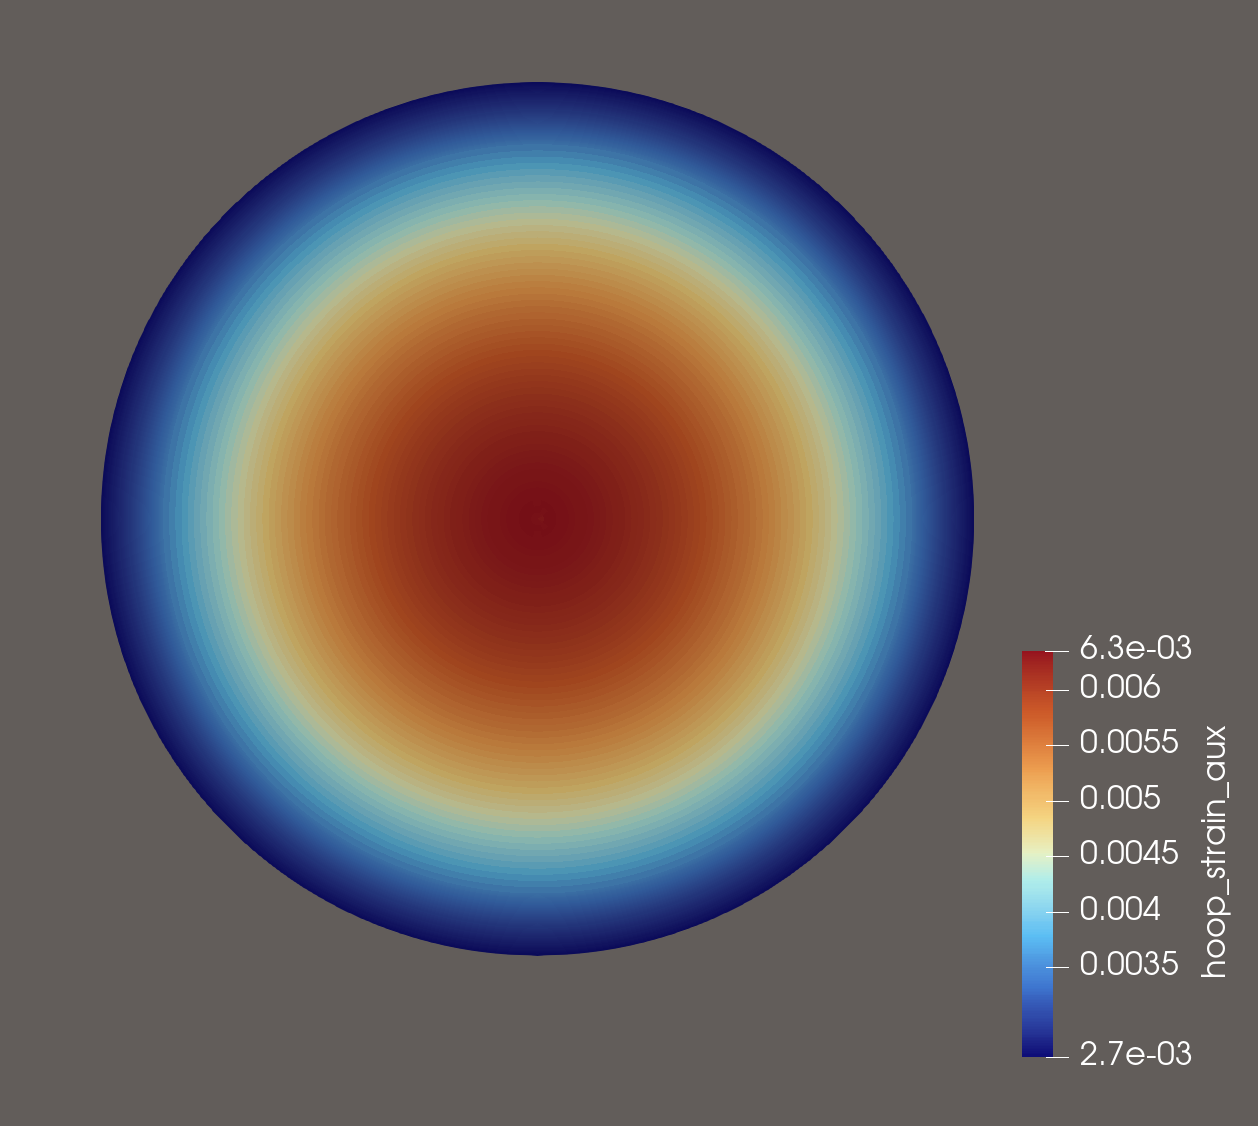
\includegraphics[width=0.5\linewidth]{figs/hoop_strain_TMI.png}
    \caption{Hoop strain profile at steady state during the operation of TMI-1.}
    \label{fig:placeholder}
\end{figure}

Displacement fields demonstrate outward radial expansion of the fuel, driven by thermal expansion. The magnitude of displacement is highest near the outer radius, indicating mechanical interaction with the cladding.

\begin{figure}[H]
    \centering
    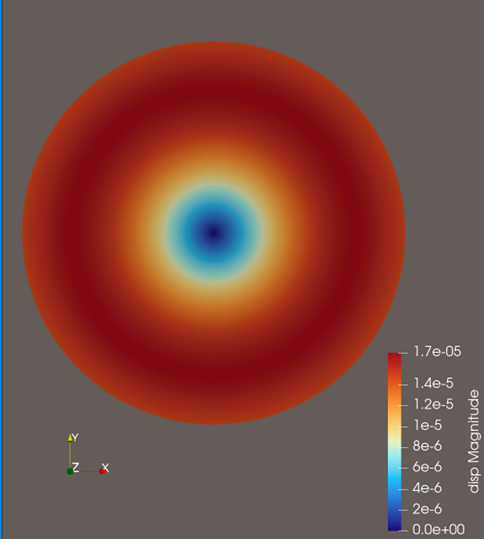
\includegraphics[width=0.5\linewidth]{figs/atomic-displacements-ss.png}
    \caption{Atomic displacements(m) of fuel and clad at steady state.}
    \label{fig:placeholder}
\end{figure}

In addition to the above variables, degradation factors specifically for the fuel and the clad were modeled as the fuel reached EOC. The conductivity and the stiffness were both degraded. These properties for the clad were also degraded simulating corrosion by the Arrhenius equation. Simultaneously, corrosion-driven degradation of the cladding further weakens its load-bearing capacity, setting the stage for failure under subsequent operating conditions.

\begin{figure}[H]
    \centering
    
\includegraphics[width=0.5\linewidth]{figs/oxidation-eoc.png}
    \caption{The oxide growth thickness (m) due to corrosion at EOC.}
    \label{fig:placeholder}
\end{figure}

\subsection{Cooling Period}
The spent fuel was simulated as cooling in a wet storage pool for 20 years. In this model, no heat source was added, and corrosion of the cladding continued. The fuel is cooled down to 340 K after 20 years. During this period, volumetric contraction occurs, and some of the compressive stress built up during heating is released. However, due to irreversible nature of prior deformation, residual stresses remain within the cladding.

Despite the reduction in temperature, corrosion continues progressing due to a long exposure time. The oxide layer on the cladding surfaces grows to be nearly 0.45 mm over the storage period. This oxide buildup contributes to further conductivity degradation of the cladding and its mechanical stiffness, reducing its load-bearing capability and causing embrittlement.

These effects together result in a structurally weaker cladding before it is reheated in the LBR cycle. Although the mechanical state of the fuel element appears to be stable, it is in a drastically degraded condition with significantly reduced safety margins.
\begin{figure}[H]
    \centering
    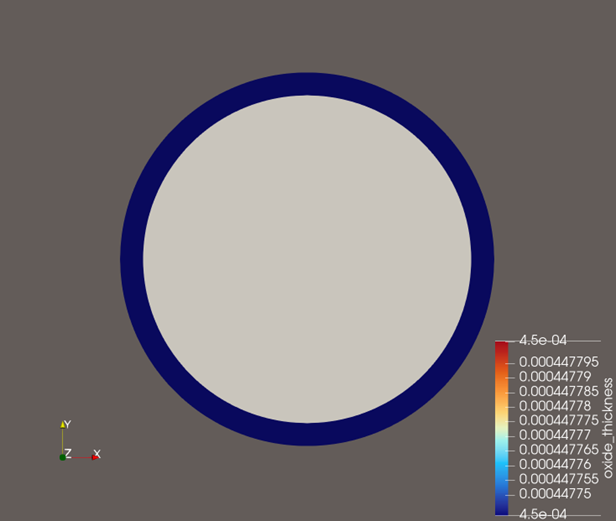
\includegraphics[width=0.5\linewidth]{figs/oxide-cool.png}
    \caption{Oxide buildup (m) on the clad surface.}
    \label{fig:placeholder}
\end{figure}

\begin{table}[H]
    \centering
    \caption{The properties for the clad before vs after heating and cooling}
    \label{tab:clad-props}
    \renewcommand{\arraystretch}{1.8}
    \begin{tabular}{>{\bfseries\raggedright\arraybackslash}m{3.8cm}
                    >{\centering\arraybackslash}m{2.5cm}
                    >{\centering\arraybackslash}m{2.8cm}}
    \toprule
    \makecell[l]{State} & \textbf{Conductivity (W/m-K)} & \textbf{Young's Modulus (Pa)}  \\
    \midrule
      Fresh & 17.0 & $1.0\times 10^{11}$ \\
      Degraded & 9.2 &  $6.9\times 10^{10}$  \\
    \bottomrule
    \end{tabular}
\end{table}

\subsection{Last Breath Reactor (Reheating Cycle)}

After the long heating and cooling periods, the spent fuel was subjected to the operating conditions of the Last Breath Reactor (LBR). The spent fuel was subjected to a volumetric heat of 305 MW/m$^3$ as derived from the thermalhydrauclics calculations, degraded conductivities of 2.5 and 9.2 W/(m-K) for the fuel and clad respectively, and a clad stiffness of 69 GPa, as obtained from the degradation mechanisms of prior simulations. Initially, for this part of the simulation, the Allen-Cahn phase field was turned on for the cladding to ensure it could survive the LBR cycle after extreme thermo-mechanical stresses. This is a genuine concern, as the LBR cycle uses a higher volumetric heat with poorer material properties, which hinders sufficient heat removal from the system, ramping up the thermal gradient and increasing the induced stresses even further.

 The thermal expansion, reduced stiffness, induced creep, and pre-existing corrosion damage cause the cladding to undergo severe thermomechanical loading. As observed by the fracture model, cracks propagate rapidly within a few days of operation. Normally, cracks are expected to propagate from the outer surface of the fuel, as shown in Figure 61 (b) for the TMI cycle, since ceramics tend to crack easily. However, cracking in Zircaloy-4, a metallic alloy, is an uncommon phenomenon that occurs directly. However, due to corrosion embrittlement and creep buildup, the cladding loses its structural integrity as a metal and begins to fracture or rupture.  

\begin{figure}[H]
    \centering
    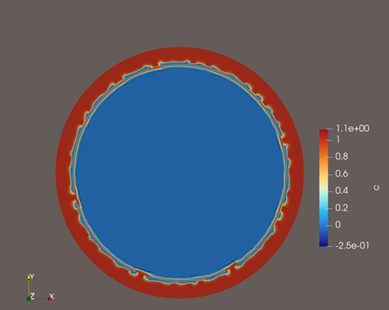
\includegraphics[width=0.49\linewidth]{figs/spent-fuel-cracks.png}
    \hfill
    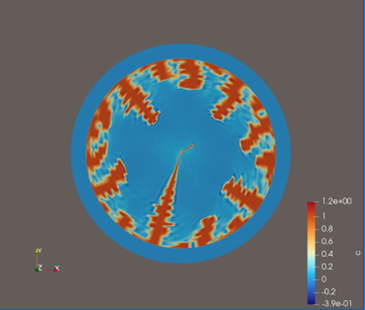
\includegraphics[width=0.49\linewidth]{figs/fresh-fuel-cracks.png}
    \caption{Crack propagation of (a) spent fuel (left) and (b) fresh fuel (right).}
    \label{fig:fuel-cracks}
\end{figure}

It should be noted that this model ignores irradiation induced damage and with the cladding already ruptured at the outer edges, there is  a significant risk, that the cracks would propagate enough, exposing the fuel region to the coolant. That would cause discharge of the fission products and gases into the coolant.

These results demonstrate that reuse of spent fuel without structural reinforcement is not viable under the aggressive thermal and mechanical environment of the LBR

\subsection{Failure Criteria and Safety Implications}

The structural integrity of the fuel–cladding system was evaluated using multiple failure criteria based on stress, creep deformation, and fracture mechanics.
Ductile failure in the cladding is assessed using the Von Mises yield criterion:
\begin{equation}
    \sigma_{vm}\geq\sigma_y
\end{equation}
where $\sigma_{vm}$ is the equivalent Von Mises stress and $\sigma_y$ is the yield strength of the material. When this condition is satisfied, plastic deformation and time-dependent creep mechanisms become dominant.
Creep rupture is further governed by the strong dependence of strain rate on stress and temperature, as previously described by the Norton–Arrhenius relation. Under elevated temperatures in the LBR cycle, even moderate stresses can lead to accelerated creep deformation, significantly reducing structural lifetime.

Meanwhile, a saturation-type corrosion model governs progressive oxide growth on the sleeve outer surface. This modulates both the elasticity and the conductivity of the sleeve. As corrosion progresses, the sleeve's conductivity degrades and raises local temperatures which accelerates creep. additionally, The degradation of conductivity and Young's modulus, substantially alters the stress redistribution at the fuel--clad interface.

Any single criterion by itself does not govern cladding failure. The simulation captures the synergistic interaction between thermally induced hoop stress, progressive creep strain accumulation in the clad, and the time-dependent stiffness reduction imposed by corrosion. Failure is considered to begin when the Von Mises stress  surpasses the  material yield strength in Zircaloy. A consequence of this is a structural lifetime limited by the rate of creep-driven strain under the degraded mechanical properties of the corroded Zircaloy. This coupled degradation route accelerates crack propagation in the cladding that highlights the need of a secondary containment system.


\subsection{Design of an Overclad}
\label{sec:overclad-design}
To prevent fuel failure through cladding rupture, the proposed solution for the last breath reactor would be to use an overclad coating. This coating layer would fit onto the clad like a sleeve. The material should be of good conductivity and high structural integrity.  The primary choice for this would be chromium, as Framatome has already been exploring chromium-coated fuel rods

\begin{figure}[H]
    \centering
    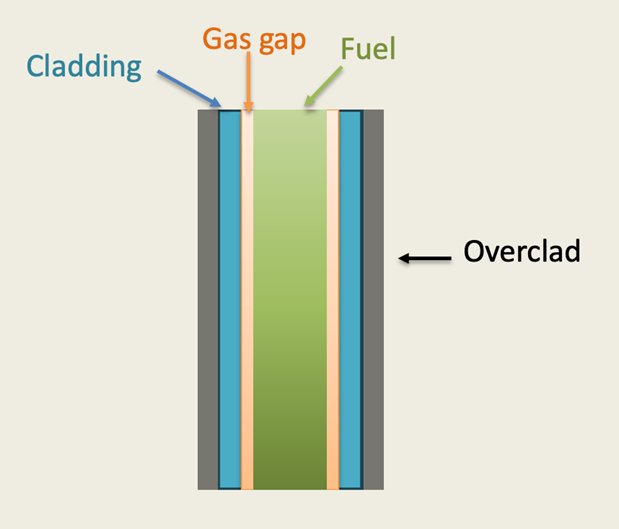
\includegraphics[width=0.5\linewidth]{figs/overclad-system.png}
    \caption{Overclad placement system.}
    \label{fig:placeholder}
\end{figure}

To choose a material for the overclad many things should be kept in mind. First and foremost, materialistic properties such as ability to withstand corrosion, the structural integrity, the penalty on neutronics, manufacturing feasibility and heat removal capabilities.

\textbf{Pure Chromium coating:}

Using a pure chromium coating, such as Framatome’s accident-tolerant fuel, would significantly improve corrosion resistance, as Chromium has an extremely low oxide pickup rate. It also has a very high thermal conductivity of 76 W/m-K at high temperatures, enabling exceptional heat transfer. However, the problem is that chromium cannot withstand the internal pressure if the cladding has already failed. The material is an exceptional coating choice for fresh fuel when the cladding has no pre-existing damage. Hence, there is a significantly high possibility that it would fail as a backup containment unit for the cladding \cite{BischoffCR-COATEDFRAMATOME}, \cite{Terrani2018AccidentChallenges}.%(Bischoff, J. et al., Framatome Chromium-Coated Zircaloy Cladding: From Development to Qualification, TopFuel 2018. The properties and ATF development context are also well documented in: Terrani, K.A., Accident Tolerant Fuel Cladding Development: Promise, Status, and Challenges, Journal of Nuclear Materials, Vol. 501, 2018. https://www.sciencedirect.com/science/article/pii/S002231151731342X)

\textbf{FeCrAl sleeve:}

The alloy of chromium mixed with iron and aluminum has quite an impressive ability to withstand internal pressure. In perfect-world conditions, this material would prove to be the ideal overclad material, as it can remove heat just as well as pure chromium. However, the biggest concern is that FeCrAl is a neutron absorber and can tax the reactor neutron  economy quite heavily thus impacting the power generation \cite{Lavrentiev2018Chromium-vacancyStudy}.

\textbf{SiC sleeve:}

The silicon carbide has a slightly poorer thermal conductivity, causing a poorer heat removal,  however it outperforms the prior choices in structural integrity, corrosion rates, and neutron economy. The biggest concern with this, however, is that it is currently quite difficult to manufacture, making it a much less feasible option \cite{Deck2015CharacterizationCladding}.

\textbf{Zircaloy-4} :

Probably one of the most conservative choices for the overcladding would be to use the cladding material itself to act as its backup containment. Having historically proven structural integrity, heat removal, and neutron economy, this material stands out the most to be the overcladding material, with the only concern being the impractical mechanisms of inserting the spent fuel into the zircaloy sleeve \cite{Motta2015CorrosionCladding}.%(Motta, A.T. et al., Corrosion of Zirconium Alloys Used for Nuclear Fuel Cladding, Annual Review of Materials Research, 2015. https://www.nuce.psu.edu/Motta/Publications/124_Motta_ARoMR_2015.pdf).


\begin{table}[H]
    \centering
    \caption{The decision-making model for overclad material selection.}
    \label{tab:decision_matrix-overclad}
    \renewcommand{\arraystretch}{1.8}
    \begin{tabular}{>{\bfseries\raggedright\arraybackslash}m{3.8cm}
                    >{\centering\arraybackslash}m{1.2cm}
                    >{\centering\arraybackslash}m{1.8cm}
                    >{\centering\arraybackslash}m{1.5cm}
                    >{\centering\arraybackslash}m{1.8cm}
                    >{\centering\arraybackslash}m{1.5cm}}
    \toprule
    \textbf{Criteria} & \textbf{Weight} & \textbf{Cr} & \textbf{FeCrAl} & \textbf{SiC} & \textbf{Zircaloy-4} \\
    \midrule
    Structural Strength        & 0.4 & 3 & 7 & 6 & 8 \\
    Neutron Economy            & 0.3 & 7 & 2 & 6 & 7 \\
    Heat Removal               & 0.2 & 9 & 8 & 5 & 6 \\
    Manufacturing Capability   & 0.1 & 6 & 6 & 2 & 4 \\
    \midrule
    \textbf{Total} & \textbf{1.0} & \textbf{5.70} & \textbf{5.6} & \textbf{5.4} & \textbf{6.9} \\
    \bottomrule
    \end{tabular}
\end{table}

The matrix weighs structural integrity as the highest (0.4) since cladding failure is the biggest concern of this simulation, as the overclad's sole function is to act as a secondary confinement layer. Neutron economy follows next (0.3), as excessive neutron absorption would penalize the reactor's already constrained fuel utilization. Heat removal was ranked next as the conductivity differences amongst the candidate materials are modest. Manufacturing capability was ranked last (0.1) despite being a real engineering problem, as it can be resolved with sufficient capital investment. Under this scheme, Zircaloy-4 scores the highest at 6.9 out of 10, primarily due to its structural strength and competitive performance across the other criteria, making it the most preferable candidate for the LBR concept.

\subsubsection{Materials testing for overclad}

In order to able to use fresh Zircaloy as the overclad, it must be ensured that it survives the conditions of the Last Breath Reactor cycle. It must be able to act as a secondary containment once the clad ruptures and holds back the fission products and the fuel particles from flowing into the coolant. Conservative guesses would assume that the overclad survives, since it is the same material as the original cladding, and since Zircaloy-4 is known to survive for an operating cycle of 5 years (which is also backed by previous simulations), it should be able to survive the smaller 300-day LBR cycle.

However, in this scenario, there is essentially no gas gap in between overclad and the cladding, and the ruptured cladding might exert additional pressure from the inside. Moreover, as the thermal simulations suggest higher temperatures for the cladding, the temperature coupled corrosion would be accelerated as well. Hence it was necessary to do the following simulations on MOOSE to make sure the overclad does not lose its structural integrity due to creep and corrosion.

\begin{figure}[H]
    \centering
    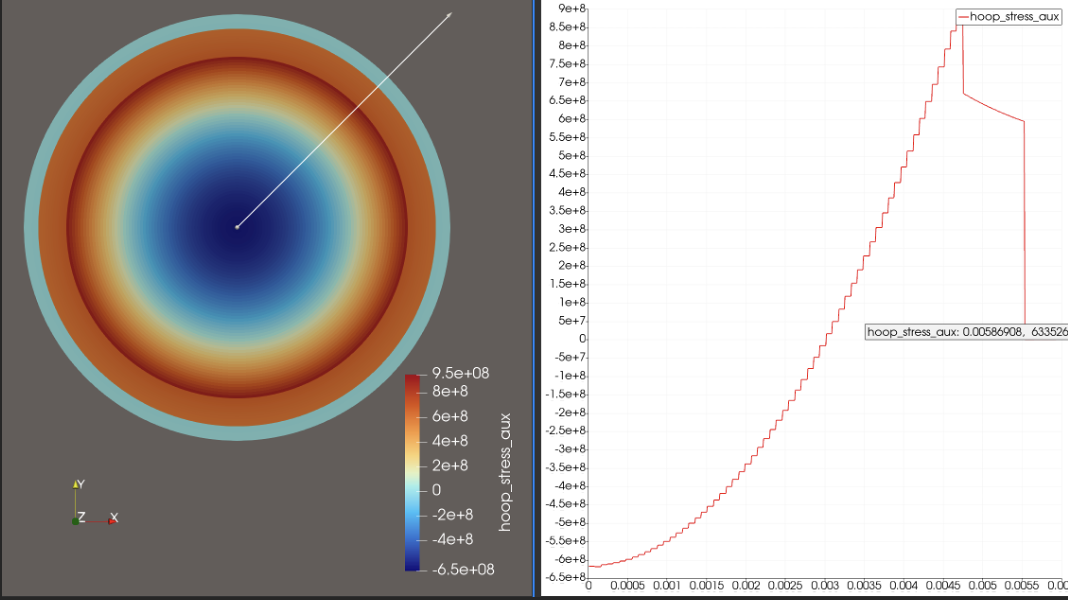
\includegraphics[width=0.8\linewidth]{figs/hoop_stress_LBR.png}
    \caption{Hoop stress (MPa) across the radial axis for the spent fuel with overclad at steady state in the Last Breath Reactor.}
    \label{fig:placeholder}
\end{figure}

\begin{table}[H]
    \centering
    \caption{The maximum hoop stress comparison between overclad and cladding in LBR vs TMI.}
    \label{tab:hoop-stress-comparison}
    \renewcommand{\arraystretch}{1.8}
    \begin{tabular}{>{\raggedright\arraybackslash}m{6cm}
                    >{\centering\arraybackslash}m{4cm}}
    \toprule
     & \textbf{Hoop Stress (MPa)} \\
    \midrule
    Fresh Zircaloy overclad in LBR & 0.633 \\
    Cladding in TMI                & 210   \\
    \bottomrule
    \end{tabular}
\end{table}

The hoop stress in the overclad is several orders of magnitude below that of the cladding in TMI. This can primarily be explained by the difference in inner pressure both elements experience. The overclad receives its inner pressure from the cladding, which is around 500~MPa for the LBR. Meanwhile in TMI, almost all the pressure the cladding receives is from the expansion of the fuel, which is around 900~MPa. In addition to PCI taking place, this significantly increases the pressure received by the cladding. The failed cladding also helps redistribute pressure from the outer clad surface onto the inner overclad surface.

\begin{figure}[H]
    \centering
    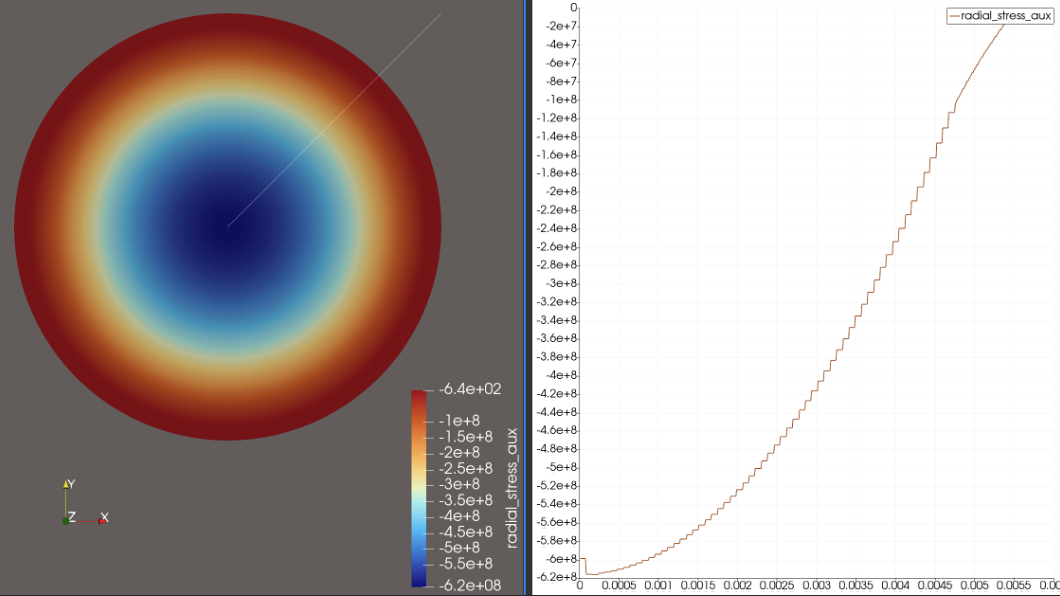
\includegraphics[width=0.8\linewidth]{figs/radial_stress_LBR.png}
    \caption{Radial stress (kPa) across the radial axis for the spent fuel with overclad at steady state in the Last Breath Reactor.}
    \label{fig:placeholder}
\end{figure}

\begin{table}[H]
    \centering
    \caption{The maximum radial stress comparison between overclad and cladding in LBR vs TMI.}
    \label{tab:radial-stress-comparison}
    \renewcommand{\arraystretch}{1.8}
    \begin{tabular}{>{\raggedright\arraybackslash}m{6cm}
                    >{\centering\arraybackslash}m{4cm}}
    \toprule
     & \textbf{Radial Stress (kPa)} \\
    \midrule
    Fresh Zircaloy overclad in LBR & 0.620 \\
    Cladding in TMI                & 210   \\
    \bottomrule
    \end{tabular}
\end{table}

Radial stress is equal to the contact pressure applied at the inner surfaces. The inner pressure from the cladding is lower in magnitude compared to the fuel inner pressure in the TMI cycle. This is further reduced due to the cracks and voids present in the ruptured cladding.

\begin{figure}[H]
    \centering
    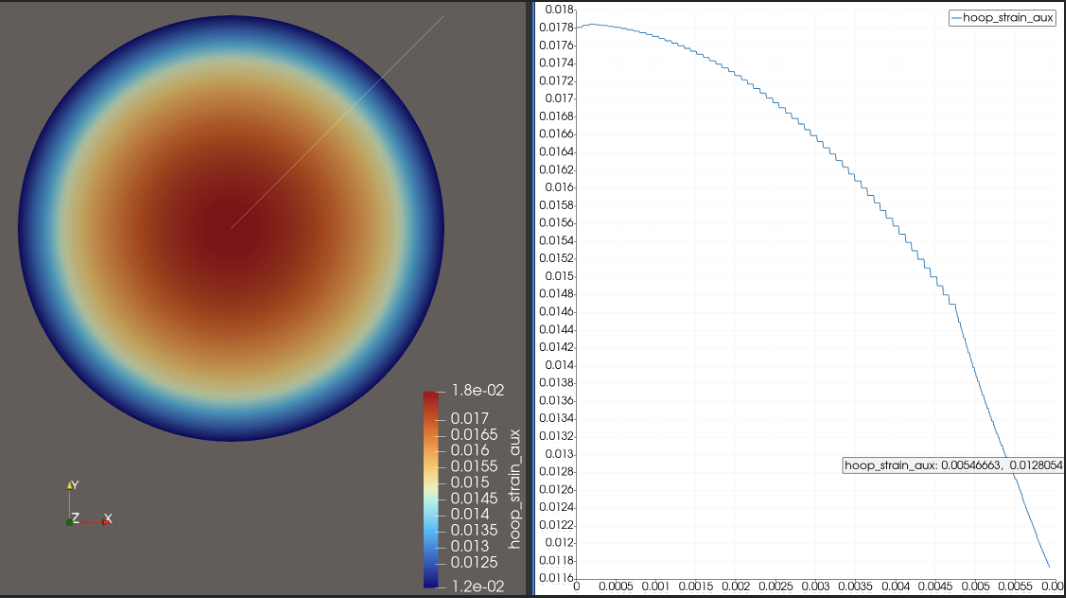
\includegraphics[width=0.8\linewidth]{figs/hoop_strain_LBR.png}
    \caption{Hoop strain across the radial axis for the spent fuel with overclad at steady state in the Last Breath Reactor.}
    \label{fig:placeholder}
\end{figure}

\begin{table}[H]
    \centering
    \caption{The maximum hoop strain comparison between overclad and cladding in LBR vs TMI at steady state.}
    \label{tab:hoop-strain-comparison}
    \renewcommand{\arraystretch}{1.8}
    \begin{tabular}{>{\raggedright\arraybackslash}m{6cm}
                    >{\centering\arraybackslash}m{4cm}}
    \toprule
     & \textbf{Hoop Strain} \\
    \midrule
    Fresh Zircaloy overclad in LBR & 0.013 \\
    Cladding in TMI                & 0.002 \\
    \bottomrule
    \end{tabular}
\end{table}

The hoop strain may appear concerning at first, as its magnitude in the overclad is higher than that of the cladding in TMI. However, the hoop strain is the sum of the creep strain, elastic strain, and thermal strain. The thermal strain, which drives thermal expansion, is considerably higher in the LBR cycle. The creep strain, governed by the Von Mises stress, is significantly lower in the overclad, as demonstrated by the following data.

\begin{figure}[H]
    \centering
    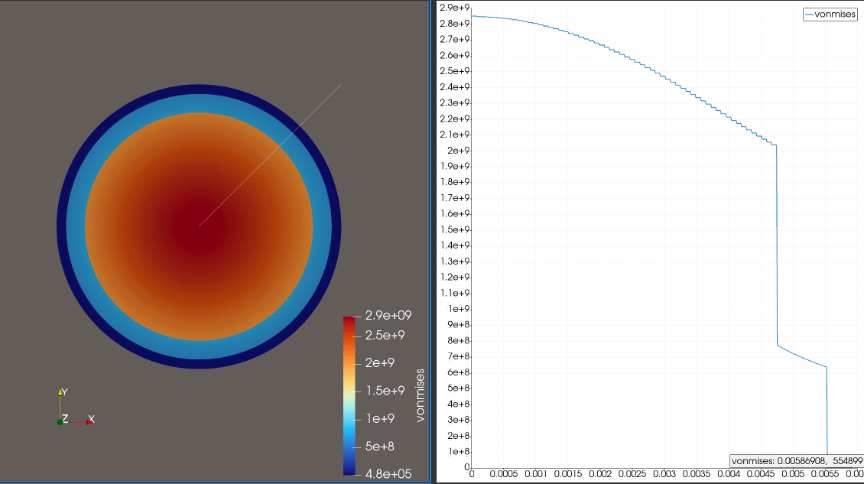
\includegraphics[width=0.8\linewidth]{figs/vonmises_LBR.png}
    \caption{Von Mises Stress (MPa) across the radial axis for the spent fuel with overclad at steady state in the Last Breath Reactor.}
    \label{fig:von-mises-overclad}
\end{figure}

\begin{table}[H]
    \centering
    \caption{Maximum Von Mises stress comparison between overclad and cladding in LBR vs TMI at steady state.}
    \label{tab:von-mises-comparison}
    \renewcommand{\arraystretch}{1.8}
    \begin{tabular}{>{\raggedright\arraybackslash}m{6cm}
                    >{\centering\arraybackslash}m{4cm}}
    \toprule
     & \textbf{Von Mises Stress (MPa)} \\
    \midrule
    Fresh Zircaloy overclad in LBR & 0.555 \\
    Cladding in TMI                & 160   \\
    \bottomrule
    \end{tabular}
\end{table}

The Von Mises stress is substantially lower for the overclad. Being the combined result of the hoop and radial stresses, the same reasoning regarding the ruptured cladding applies here. The lower Von Mises stress in the LBR overclad compared to the TMI cladding further ensures that the overclad will undergo significantly less creep and will maintain structural integrity over the 300-day operating cycle.

\begin{figure}[H]
    \centering
    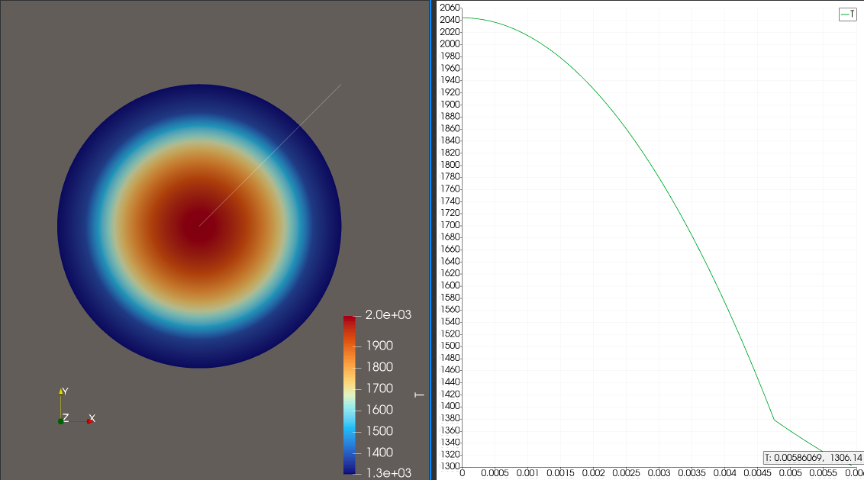
\includegraphics[width=0.8\linewidth]{figs/temp_LBR.png}
    \caption{Radial temperature profile (K) for the spent fuel with overclad at steady state in the Last Breath Reactor.}
    \label{fig:placeholder}
\end{figure}

\begin{table}[H]
    \centering
    \caption{Outermost edge temperature comparison between overclad and cladding in LBR vs TMI at steady state.}
    \label{tab:temp-comparison}
    \renewcommand{\arraystretch}{1.8}
    \begin{tabular}{>{\raggedright\arraybackslash}m{6cm}
                    >{\centering\arraybackslash}m{4cm}}
    \toprule
     & \textbf{Temperature (K)} \\
    \midrule
    Fresh Zircaloy overclad in LBR & 1306 \\
    Cladding in TMI                & 420  \\
    \bottomrule
    \end{tabular}
\end{table}

The overclad temperature is roughly three times higher than the clad temperature in TMI. This is due to a higher volumetric heat source being used with a poorer model of heat removal than that present in the TMI cycle. As corrosion is significantly sped up in higher temperatures, and operating in a long cycle would generally worsen the materials elasticity, the high temperature does raise a doubt in terms of overclad safety. However, these spent fuel rods will be under operation for 300 days in comparison to 5 years, so it would undergo less corrosion which is backed by the simulations data. On the other hand, the 1306K is under the NRC limit of 10 CFR 50.46, so no regulatory limits are being breached in this scenario \cite{NRC_50_46}. However, it must be noted that Zircaloy undergoes significant strength reduction at high temperatures. At room temperatures, the material has a yield strength of 500 MPa while reducing down to 100-150 MPa in the 1300 K temperature range \cite{NUREG/CR-6739Rods.}. Nevertheless, the Von Mises stress is only 0.555 MPa in the overclad, quite significantly below the yield strength ensuring the material is well within its elastic limit and is not in the risk of plastic collapse.%(Geelhood, K.J. and Luscher, W.G., FRAPTRAN-2.0: A Computer Code for the Transient Analysis of Oxide Fuel Rods, PNNL-19400, NRC, 2015. The material property models in this code document the temperature-dependent yield strength of Zircaloy-4. https://www.nrc.gov/docs/ML1611/ML16118A413.pdf)

\begin{figure}[H]
    \centering
    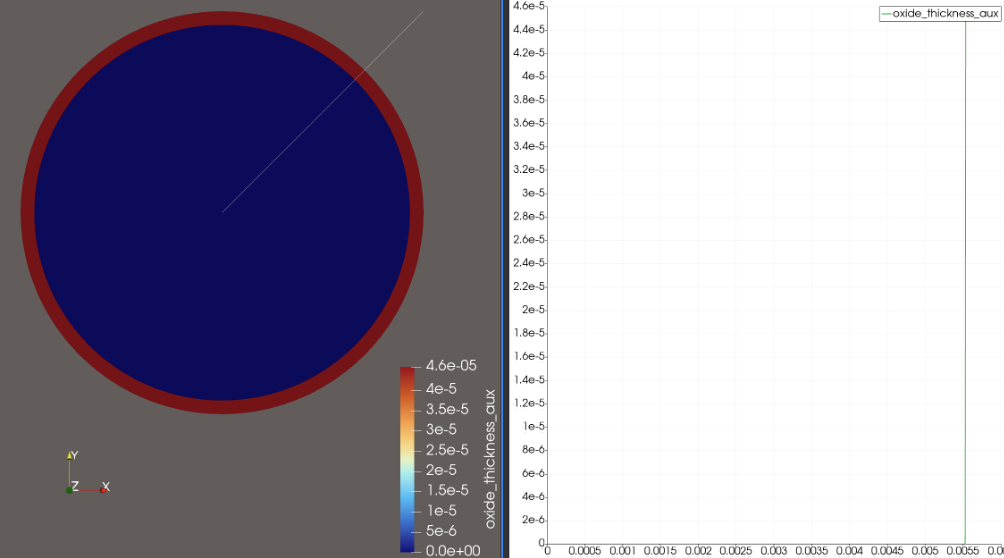
\includegraphics[width=0.8\linewidth]{figs/corrosion_LBR.png}
    \caption{Oxide growth (mm) across the radial axis for the spent fuel with overclad at steady state in the Last Breath Reactor.}
    \label{fig:placeholder}
\end{figure}

\begin{table}[H]
    \centering
    \caption{Oxide growth thickness comparison between overclad and cladding in LBR vs TMI at steady state.}
    \label{tab:oxide-growth-comparison}
    \renewcommand{\arraystretch}{1.8}
    \begin{tabular}{>{\raggedright\arraybackslash}m{6cm}
                    >{\centering\arraybackslash}m{4cm}}
    \toprule
     & \textbf{Oxide Growth (mm)} \\
    \midrule
    Fresh Zircaloy overclad in LBR & 0.046 \\
    Cladding in TMI                & 0.065 \\
    \bottomrule
    \end{tabular}
\end{table}

Although the elevated overclad temperature accelerates corrosion kinetics, the shorter 300-day LBR cycle results in less total oxide growth (0.046~mm) compared to the TMI cladding (0.065~mm). The risk of embrittlement-driven failure is therefore lower for the overclad, given that standard PWR cladding does not typically fail under the corrosion damage accumulated during a normal operating cycle.

\paragraph{Engineering Interpretation}

The introduction of a Zircaloy-4 overclad fundamentally alters the stress distribution within the fuel system by acting as a secondary structural barrier. In the absence of a gap, mechanical loads from the degraded cladding are directly transferred to the overclad, resulting in increased contact stresses. However, due to its intact mechanical properties, the overclad is capable of redistributing these stresses and preventing catastrophic failure.

Despite elevated temperatures and ongoing corrosion, the overclad maintains structural integrity throughout the LBR cycle, as indicated by the relatively low Von Mises stress compared to expected yield limits. This demonstrates that the overclad effectively compensates for the loss of strength in the original cladding.

These results suggest that the use of a Zircaloy-4 sleeve is a viable strategy for extending the operational lifetime of spent fuel under high-power conditions, provided that manufacturing and assembly challenges can be addressed.



\subsection{Model Validation and Physical Consistency}

To ensure the reliability of the simulation results, key outputs were compared against expected physical behavior and values reported in the literature.

The predicted centerline temperatures of $\sim$1100~K during the primary cycle are consistent with typical PWR fuel operating conditions, as reported in the nominal value of 1070~K in the Westinghouse PWR Systems Manual \cite{WestinghouseLimits}, %(NRC/Westinghouse Technology Systems Manual, Section 2.2, ML11223A208. https://www.nrc.gov/docs/ml1122/ML11223A208.pdf). 
 and are comparable to the 950--1150~K range validated by the FRAPCON-4.0 fuel performance code at similar power densities %(Geelhood, K.J. et al., FRAPCON-4.0: A Computer Code for the Calculation of Steady-State Thermal-Mechanical Behavior of Oxide Fuel Rods, PNNL-19418 Vol. 2 Rev. 2, NRC. https://www.nrc.gov/docs/ML1611/ML16118A434.pdf)
 \cite{2015FRAPCON-4.0Assessment.}. Likewise, the hoop stress distributions agree with the established PCMI behavior reported in the ORNL fuel cracking analysis \cite{Sweet2018AnalysisRelocation}, %(ORNL/TM-2018/889, Analysis of FeCrAl Cladding and UO₂ Fuel Including Discrete and Smeared Cracks. https://info.ornl.gov/sites/publications/Files/Pub112359.pdf
  and the maximum cladding hoop stress of 210~MPa lies within the 150--666~MPa range reported for PWR fuel rods \cite{Qi2020Pellet-claddingCladding}.%(Sercombe, J. et al., Pellet-cladding mechanical interaction analysis of Cr-coated Zircaloy cladding, Nuclear Engineering and Design, 2020. https://www.sciencedirect.com/science/article/pii/S0029549320302867).

The observed temperature increase during the LBR cycle is physically consistent with reduced thermal conductivity due to fuel degradation, combined with a higher volumetric heat source and reduced convective heat removal. The Arrhenius corrosion model aligns well with experimental data on PWR Zircaloy-4, where corrosion kinetics follow a cubic rate law with an activation energy of 132.8~kJ/mol \cite{osti_23002966}. %(Sato, T. et al., Autoclave Corrosion Experiment of Zircaloy-4 at Temperatures Between 180°C and 270°C, WM2019 Conference Proceedings, OSTI:23002966. https://www.osti.gov/biblio/23002966).
 Furthermore, the thermally driven corrosion behavior during the 20-year cooling period is consistent with established Zircaloy corrosion literature \cite{Motta2015CorrosionCladding}. %Motta, A.T. et al., Corrosion of Zirconium Alloys Used for Nuclear Fuel Cladding, Annual Review of Materials Research, 2015.: https://www.nuce.psu.edu/Motta/Publications/124_Motta_ARoMR_2015.pdf).

The predicted failure mode, characterized by cladding-initiated cracking driven by corrosion embrittlement, creep, and degraded material properties under high-temperature conditions, agrees with experimental observations on Zircaloy-4, where waterside corrosion produces a brittle hydride rim with significantly reduced fracture resistance under the multi-axial stress states induced during the LBR reheating cycle \cite{ONReader}. %(Daum, R.S. et al., On the Embrittlement of Zircaloy-4 under RIA-Relevant Conditions, ANL, 2001. https://publications.anl.gov/anlpubs/2001/12/41627.pdf)

Overall, the model captures the dominant physical mechanisms governing fuel--cladding behavior and provides results consistent with known reactor materials performance trends.

\subsection{Limitations and Future Work}

While the present model captures the key thermo-mechanical and degradation phenomena, several simplifying assumptions were made that may influence the accuracy of the results.

First, irradiation-induced effects such as swelling, fission gas release, and radiation hardening were not included. Neglecting fission gas pressure buildup in particular alters the hoop stress distribution. While these effects are secondary to thermo-mechanical stresses at the beginning of life, they become non-negligible at the end of the cycle. FRAPCON simulations of comparable PWR fuel rods indicate that internal fission gas pressure at the end of the cycle can contribute an additional 50--100~MPa of hoop stress to the cladding \cite{2015FRAPCON-4.0Assessment.}, %(Geelhood, K.J. et al., FRAPCON-4.0: A Computer Code for the Calculation of Steady-State Thermal-Mechanical Behavior of Oxide Fuel Rods, PNNL-19418 Vol. 2 Rev. 2, NRC. https://www.nrc.gov/docs/ML1611/ML16118A434.pdf).
 meaning the LBR cladding and overclad stresses are likely underestimated.

Additionally, the corrosion model is simplified and does not account for complex oxide layer behavior, such as spallation or transition kinetics. The exclusion of these phenomena results in an underestimate of the peak corrosion rates of Zircaloy in reactor conditions as corrosion rates are known to accelerate to a factor of 6 when fuel undergoes multiple irradiation cycles %(Blat, M. and Noel, D., Analysis of the Waterside Corrosion Kinetics of Zircaloy-4 Fuel Cladding in French PWRs, Nuclear Technology, Vol. 170, 2010.  https://www.tandfonline.com/doi/abs/10.13182/NT10-A10330)
\cite{Bouineau01062010}. The phase-field fracture model, while effective in capturing crack propagation, does not explicitly resolve microstructural mechanisms such as grain boundary failure.

Ignoring the fuel gas gap in the primary cycle simulates the fuel having more heat removal than normal, resulting in a much cooler fuel as it is the strongest element of thermal resistance. This means that the model assumes direct conductive contact across the fuel–cladding interface, artificially enhancing heat removal from the fuel and resulting in a non-conservative underestimate of the fuel centerline temperature %(Lapetite, J.M. et al., Measurement of the Thermal Conductivity of Metal Clad Uranium Oxide Rods During Irradiation, Journal of Nuclear Materials, 1961. https://www.sciencedirect.com/science/article/abs/pii/0022311561902021)
\cite{Cohen1961MeasurementIrradiation}. However, it should be addressed that the gas gap limitation applies to the primary heating cycle and during the LBR heating phase, the ruptured cladding is in direct contact with the overclad, which makes the no gas-gap assumption an approximation that is much closer to reality for that stage of the simulation.

Future work should include irradiation effects with detailed neutron fluence data, burnup tracking and DPA (displacement per atom) evolutions, which would allow to simulate DPA correlations, swelling laws and irradiation creep coefficients that can be cross-checked with more advanced models such as BISON or FRAPCON. With the availability of sufficient computational power, these simulations can be rerun with the more advanced corrosion kinetics, a detailed phase field fracture physics and including gap mechanics.